\def\year{2020}\relax
%File: formatting-instruction.tex
\documentclass[letterpaper]{article} % DO NOT CHANGE THIS
\usepackage{aaai20}  % DO NOT CHANGE THIS
\usepackage{times}  % DO NOT CHANGE THIS
\usepackage{helvet} % DO NOT CHANGE THIS
\usepackage{courier}  % DO NOT CHANGE THIS
\usepackage[hyphens]{url}  % DO NOT CHANGE THIS
\usepackage{graphicx} % DO NOT CHANGE THIS
\urlstyle{rm} % DO NOT CHANGE THIS
\def\UrlFont{\rm}  % DO NOT CHANGE THIS
\usepackage{graphicx}  % DO NOT CHANGE THIS
\frenchspacing  % DO NOT CHANGE THIS
\setlength{\pdfpagewidth}{8.5in}  % DO NOT CHANGE THIS
\setlength{\pdfpageheight}{11in}  % DO NOT CHANGE THIS
%\nocopyright
%PDF Info Is REQUIRED.
% For /Author, add all authors within the parentheses, separated by commas. No accents or commands.
% For /Title, add Title in Mixed Case. No accents or commands. Retain the parentheses.
% \pdfinfo{
%/Title (AAAI Press Formatting Instructions for Authors Using LaTeX -- A Guide)
%/Author (AAAI Press Staff, Pater Patel Schneider, Sunil Issar, J. Scott Penberthy, George Ferguson, Hans Guesgen)
} %Leave this	
% /Title ()
% Put your actual complete title (no codes, scripts, shortcuts, or LaTeX commands) within the parentheses in mixed case
% Leave the space between \Title and the beginning parenthesis alone
% /Author ()
% Put your actual complete list of authors (no codes, scripts, shortcuts, or LaTeX commands) within the parentheses in mixed case. 
% Each author should be only by a comma. If the name contains accents, remove them. If there are any LaTeX commands, 
% remove them. 

\usepackage[dvipsnames]{xcolor}

% DISALLOWED PACKAGES
% \usepackage{authblk} -- This package is specifically forbidden
% \usepackage{balance} -- This package is specifically forbidden
% \usepackage{caption} -- This package is specifically forbidden
% \usepackage{color (if used in text)
% \usepackage{CJK} -- This package is specifically forbidden
% \usepackage{float} -- This package is specifically forbidden
% \usepackage{flushend} -- This package is specifically forbidden
% \usepackage{fontenc} -- This package is specifically forbidden
% \usepackage{fullpage} -- This package is specifically forbidden
% \usepackage{geometry} -- This package is specifically forbidden
% \usepackage{grffile} -- This package is specifically forbidden
% \usepackage{hyperref} -- This package is specifically forbidden
% \usepackage{navigator} -- This package is specifically forbidden
% (or any other package that embeds links such as navigator or hyperref)
% \indentfirst} -- This package is specifically forbidden
% \layout} -- This package is specifically forbidden
% \multicol} -- This package is specifically forbidden
% \nameref} -- This package is specifically forbidden
% \natbib} -- This package is specifically forbidden -- use the following workaround:
% \usepackage{savetrees} -- This package is specifically forbidden
% \usepackage{setspace} -- This package is specifically forbidden
% \usepackage{stfloats} -- This package is specifically forbidden
% \usepackage{tabu} -- This package is specifically forbidden
% \usepackage{titlesec} -- This package is specifically forbidden
% \usepackage{tocbibind} -- This package is specifically forbidden
% \usepackage{ulem} -- This package is specifically forbidden
% \usepackage{wrapfig} -- This package is specifically forbidden
% DISALLOWED COMMANDS
% \nocopyright -- Your paper will not be published if you use this command
% \addtolength -- This command may not be used
% \balance -- This command may not be used
% \baselinestretch -- Your paper will not be published if you use this command
% \clearpage -- No page breaks of any kind may be used for the final version of your paper
% \columnsep -- This command may not be used
% \newpage -- No page breaks of any kind may be used for the final version of your paper
% \pagebreak -- No page breaks of any kind may be used for the final version of your paperr
% \pagestyle -- This command may not be used
% \tiny -- This is not an acceptable font size.
% \vspace{- -- No negative value may be used in proximity of a caption, figure, table, section, subsection, subsubsection, or reference
% \vskip{- -- No negative value may be used to alter spacing above or below a caption, figure, table, section, subsection, subsubsection, or reference
\usepackage{mathtools}
\newcommand{\samsays}[1]{\textcolor{RubineRed}{[Sam: #1]}}
\newcommand{\yangsays}[1]{\textcolor{Blue}{[Yang: #1]}}
\newcommand{\azsays}[1]{\textcolor{Green}{[az: #1]}}
% \newcommand{\prepad}{\hspace{1.5em}}
% \newcommand{\prepadmini}{\hspace{1em}}
\newcommand{\prepad}{}
\newcommand{\bx}{\mathbf{x}}
\newcommand{\bm}{\mathbf{m}}
\newcommand{\bv}{\mathbf{v}}
\newcommand{\prepadmini}{}
\setcounter{secnumdepth}{0} %May be changed to 1 or 2 if section numbers are desired.

% The file aaai20.sty is the style file for AAAI Press 
% proceedings, working notes, and technical reports.
%
\setlength\titlebox{2.5in} % If your paper contains an overfull \vbox too high warning at the beginning of the document, use this
% command to correct it. You may not alter the value below 2.5 in
% \title{Instance-centric Video Understanding}
% \title{The Fast Cross-Modal Filter for Video Representation}
% \title{A fast cross-modal filtering architecture for video representation}
\title{Efficient cross-modal enhancement for video retrieval and classification}
%Your title must be in mixed case, not sentence case. 
% That means all verbs (including short verbs like be, is, using,and go), 
% nouns, adverbs, adjectives should be capitalized, including both words in hyphenated terms, while
% articles, conjunctions, and prepositions are lower case unless they
% directly follow a colon or long dash
\author{Anonymous Submission\\ 
Paper ID: 5269
% use superscripts in text and roman font to identify them. For example, Sunil Issar,\textsuperscript{\rm 2} J. Scott Penberthy\textsuperscript{\rm 3} George Ferguson,\textsuperscript{\rm 4} Hans Guesgen\textsuperscript{\rm 5}. Note that the comma should be placed BEFORE the superscript for optimum readability
}
 \begin{document}

\maketitle

\begin{abstract}
% In this work, we investigate the Cross Modal Filter, a technique which aims to exploit signal in one modality to resolve ambiguities in another. 
The objective of this work is video representation---we seek to compress the high-dimensional, dynamic content of a video into a compact, fixed-size vector that enables efficient retrieval and content classification.  The key idea underpinning our approach is \textit{Cross-Modal Enhancement} (CME), the technique of exploiting the context provided by signals in one modality to resolve ambiguities within another when forming the video embedding.  We investigate several instantiations of this core idea, charting the design space of different cross-modal enhancement mechanisms which trade-off computational complexity against performance.  We demonstrate the general applicability of cross-modal enhancement on different video understanding tasks: text-video retrieval and very large-scale action recognition. In the retrieval setting, we establish state-of-the-art performances on four standard benchmarks: ActivityNet, MSR-VTT, LSMDC and DiDeMo.  We then further establish the effectiveness of our approach for the task of video classification on the recently proposed Multi-Moments-in-Time benchmark.  
\end{abstract}   
\section{Introduction}


\begin{figure}
    \centering
    \includegraphics[width=0.4\textwidth]{example-image-a}
    \caption{\textbf{The Cross-Modal Filter}: Ambiguities in one sensory signal are resolved by reference to other modalities.}
    \label{fig:my_label}
\end{figure}


The objective of this work is video representation---we seek to
compress the content of a video clip into an embedding that enables
retrieval and content classification.  For practical usage, an
effective video representation has two key desiderata: (1) it should
be \textit{discriminative} for the task of interest; and (2) it should be
\textit{compact} to enable efficient storage and retrieval for very large-scale data sets.  In this
work, we develop a neural  architecture that meets both objectives.  At the
core of our method is a technique we term \textit{Cross-Modal
Enhancement}, a learnable mechanism for exploiting contextual
information from a collection of modality signals to render them
maximally discriminative for a given objective.  The design use of such a technique is motivated by the following hypothesis: \textit{information
provided by a single modality signal exhibits ambiguity which
may only be resolved through its combination with other 
signals}.  

The task of text-video retrieval requires a system to rank a
collection of videos according to how well they match a given text
query.  Joint video-text embeddings (which seek to map videos and text
descriptions into a common space such that matching video and text
pairs are close together) form an attractive model for tackling this
problem, since they readily allow for efficient indexing: compact
video embeddings can be pre-computed and stored offline such that the
test time query reduces to simple distance computation between
embeddings. The distance computation can be carried out very efficiently
and at large scale using approximate nearest neighbors (ANN)  methods.
In turn, by requiring that the video and query-text embeddings are close,
this model determines the loss for discriminatively training the video representation.
Similarly,  the task of video content classification also determines a loss 
for discriminatively training the video representation.

We consider the multiple modalities and information sources that are
available in a video clip. These include those available from the
video stream, such as human actions and faces, the objects, animals,
and scene-text, as well as the surrounding scene; and also those available
from the audio stream, such as human speech and ambient sounds.
The video representation must combine information from all of these sources and modalities in a discriminative
and compact manner.

The question then is: how should these multiple modalities be combined into the video-clip representation?
In this work we build on the MoEE/CENet joint text-video embedding
architecture initially proposed by \cite{miech2018learning} and
recently extended by \cite{liu2019use}.  This architecture (henceforth
referred to as CENet)  integrates the multiple modalities into a single video representation by computing 
{\em all}  pairwise relations between modalities. With so many modalities, computing all pairwise relations becomes
very expensive.

In this paper we investigate other architectures for combining the multiple modalities. We
 show that it is {\em not} necessary to compute all pairwise
relations to produce an effective `Cross-Modal Filtering'; rather a simple star topology graph (comparing all
modalities to a careful composed aggregate), not only significantly reduces the cost, but also leads to a more powerful representation.
Indeed, we show that using this representation exceeds the state of the art performance on the benchmarks used
by~\cite{miech2018learning} and~\cite{liu2019use}.

In this paper we make the following contributions:
\begin{enumerate}
\item We develop and evaluate a novel Cross-Modal Filtering module for effectively composing streams for video representation.
\item We present an efficient approximation to this scheme, suitable for the very-large scale video retrieval and 
content classification  settings.
\item We set a new state-of-the-art performance on four benchmarks for retrieval, as well as content classification 
on the newly proposed Multi-Moments-In-Time dataset.
\end{enumerate}

% ** original text below here **
% The objective of this work is video representation---we seek to compress the content of a video into an embedding that enables retrieval and content classification.  For practical usage, an effective video representation has two key desiderata: (1) it should be \textit{discriminative} for the task of interest; (2) it should be \textit{compact} to enable efficient storage and retrieval.  In this work, we develop an architecture that meets both objectives.   At the core of our method is a technique we term \textit{Cross-Modal Filtering}, a learnable mechanism for exploiting contextual information from a collection of sensory signals to render them maximally discriminative for a given objective.  The design of such a filter is motivated by the following hypothesis: \textit{information provided by a single modality sensory signal exhibits ambiguity which may only be resolved through its combination with other sensory signals}.  This ambiguity resolution requires the creation of representations that cannot exist at the level of individual sensors, necessitating the design of an appropriate integration system.  An example of this form of multi-modal integration can be found in the human vestibular system, in which the signal provided by the otolith organs (which detect linear acceleration) are necessarily combined with additional visual and/or semicircular canal cues to solve for transnational motion~\cite{green2010multisensory}.


% \color{red}

% \begin{itemize}
%     \item The aim of this work is large scale video understanding
%     \item We specifically focus on making good use of modalities in a manner that is practical for large scale systems
%     \item We explore designs of cross-modal filters for fusing sensory signals appropriately
%     \item We show that by including cross-modal filters in multi-modal video understanding systems, we can improve performance on multiple benchmarks. 
% \end{itemize}

% \color{black}



% \color{red}
% Motivating examples for video understanding tasks (could do with some upgrading later): 

% \begin{itemize}
%     \item We watch two humans talking, but it is only by understanding the content of their speech that we may hope to grasp the full nature of their interaction.
%   \item We see a clip of a small gathering of people, but it is only reading the text on their placards that we realise that the scene depicts a political protest.
%   \item We hear animal noises, but require visual cues to differentiate a zoo from the jungle or a veterinary office.
% \end{itemize}

% \color{black}

% \color{red}
% \begin{enumerate}
% \item We develop and evaluate a novel Cross-Modal Filtering module for effectively composing streams for video representation.
% \item We present an efficient approximation to this scheme, suitable for the very-large scale video understanding setting.
% \item We set a new state-of-the-art performance on four benchmarks for retrieval, as well as on the newly proposed Multi-Moments-In-Time dataset.
% \end{enumerate}
% \color{black}
\section{Related Work}

\subsection{Multi-Modal Embedding for Video Understanding}

Multi-modal embedding focuses on using various modalities of the sensory signal to improve the performance of a specific task. Most state-of-the-art video representations \cite{feichtenhofer2016convolutional,feichtenhofer2017spatiotemporal,simonyan2014two,miech2017learnable,wang2016temporal} separate videos into multiple stream of modalities. The appearance and motion features  \cite{feichtenhofer2016convolutional,simonyan2014two,carreira2017quo,girdhar2017actionvlad,varol2017long} capturing visual cues and audio signal \cite{miech2017learnable,monfortmoments} are the commonly used video modalities. Most recently, \cite{miech2018learning,liu2019use} leverage and combine additional cues from the video and learn the joint embedding using the context gating mechanisms. These literature has consistently demonstrated the benefits of combining different video modalities for video understanding. Similar to previous work in video understanding, our model combines multiple modalities but make it more compact to enable efficient storage and retrieval for very large-scale datasets. The proposed approach can be easily generalised a large number of modalities to leverage the rich and varied multi-modality information in video, including some fine-grained information, i.e., face, speech, OCR, etc. 

% \subsection{Action Recognition and VideO Retrieval}
% For video understanding applications, a large number of existing works focused on aggregation of single modality representations over time\cite{}, however, they ignored to leverage the rich and varied multi-modality information in video, including motion cues, speech, OCR information etc.   

% More recently, \cite{monfortmoments} attempted to fuse the multi-modality features in video by ensembling the top performing model of each modality and feature concatenation. However, the relationships among multi-modality data have not been fully explored. To utilise the expert model of each single modality, \cite{miech2018learning} proposed to learn a joint embedding built on the conventional Mixtures-of-Experts model \cite{}. The later extension \cite{liu2019use} 

% learn a joint embedding exploiting the complementary and redundant information from the heterogeneous modalities. 
% % how to represent and summarise multi-modal data in a way that exploits the complementarity and redundancy of multiple modalities. 
% A range of prior work has proposed to jointly embed images and text into the same space [17, 18, 19, 28, 38], enabling cross-modal retrieval. 
% More recently, several works have also focused on audio-visual cross-modal embeddings [2, 37], as well as audio-text embeddings [7]. Our goal in this work, however, is to embed videos and natural language sentences (sometimes multiple sentences) into the same semantic space, which is made more challenging by the high dimensional content of videos.

\subsection{Action Recognition and Video-Text Retrieval}
There exists a range of works focusing on video-text retrieval, they either chose to learn spatial-temporal visual features only \cite{otani2016learning,dong2016word2visualvec} or adopted to learn the joint embedding from multi-modality signals \cite{miech2018learning,liu2019use,mithun2018learning}. However, our method investigates the efficient architectures to combine multi-modality features for video-text retrieval task. 

Recent work on action recognition first learn compact representations across time or modalities and then perform various aggregation methods for the recognition. Another line of work \cite{wang2018videos,ma2018attend} focused more on modelling the relationship or interactions between different object instances in space and time. These methods only explored only spatial-temporal and audio features using the conventional classification formulation. However, our method attempts to utilize the powerful multi-modality joint embedding and reformulate the action recognition problem using the video-text retrieval method.
 





\section{Cross Modal Enhancement}

In this section, we introduce the Cross-Modal Enhancement and describe its role for video understanding tasks.

% \azsays {The following is too vague: here you need to give some idea of the modality-specific signals (e.g. speech, scene-text, faces) and very important - the time interval over which you are combining modalities (and creating the representation from), e.g. a video clip.}

\subsection{Resolving modality-specific ambiguities through filtering}

The objective of Cross-Modal Enhancement (CME) is to transform a collection of modality-specific video signals $\{\bm_i \}_{i \in \mathcal{M}}$ so as to render them maximally discriminative for a given task.  While these signals may be generic, the focus of this work is on high-level video understanding tasks, namely text-video retrieval and action recognition---consequently the set of signals under consideration include examples such as human speech and scene-text.  In the description that follows, we assume that that each such signal, $\bm_i$, takes the form of a fixed-size embedding (and therefore that temporal aggregation of each signal has been performed upstream).  The functional form of Cross-Modal Enhancement comprises a pair of functions: a \textit{filter generator}, $f_\phi$, the \textit{application function}, $a_\theta$, which are composed as follows:

\begin{align}
    \text{CME}(\bm_i) = a_\theta (\bm_i,  f_\phi (\{\bm_j: j \in \mathcal{N}_i\}))
    \label{eqn:cmf}
\end{align}

Here $\mathcal{N}_i$ denotes the \textit{filtering neighbourhood} of signal $\bm_i$, namely the signals which are used to generate its enhancement filter.  Cross-Modal Enhancement can thus be decomposed into its three components: (1) the selection of the filtering neighbours set, $\mathcal{N}_i$; (2) the choice of filter generator, $f_{\phi}$; (3) the design of the application function, $a_\theta$.  We discuss these choices below.

\subsubsection{Filtering Neighbourhoods:} A natural choice for the filtering neighbourhood of each input is simply the set of all signals (the filter sets therefore correspond to a dense graph, in which the signals are nodes and the edges define the neighbourhood inclusion relation).  Should prior knowledge about the relationships between the signals be available, it can be encoded directly into the filtering neighbours by imposing appropriate sparsity constrains on the inclusion graph.  In this work, we consider only small numbers of modality-specific signals and we therefore simply opt to use all possible nodes for each filtering neighbourhood, deferring further investigations of graph structure for large numbers of signals to future work.  Nevertheless, note that even dense inclusion graphs can be made computationally tractable with the appropriate choice of filter generator function---we describe this design choice next.


\begin{figure}[t]
\begin{center}
        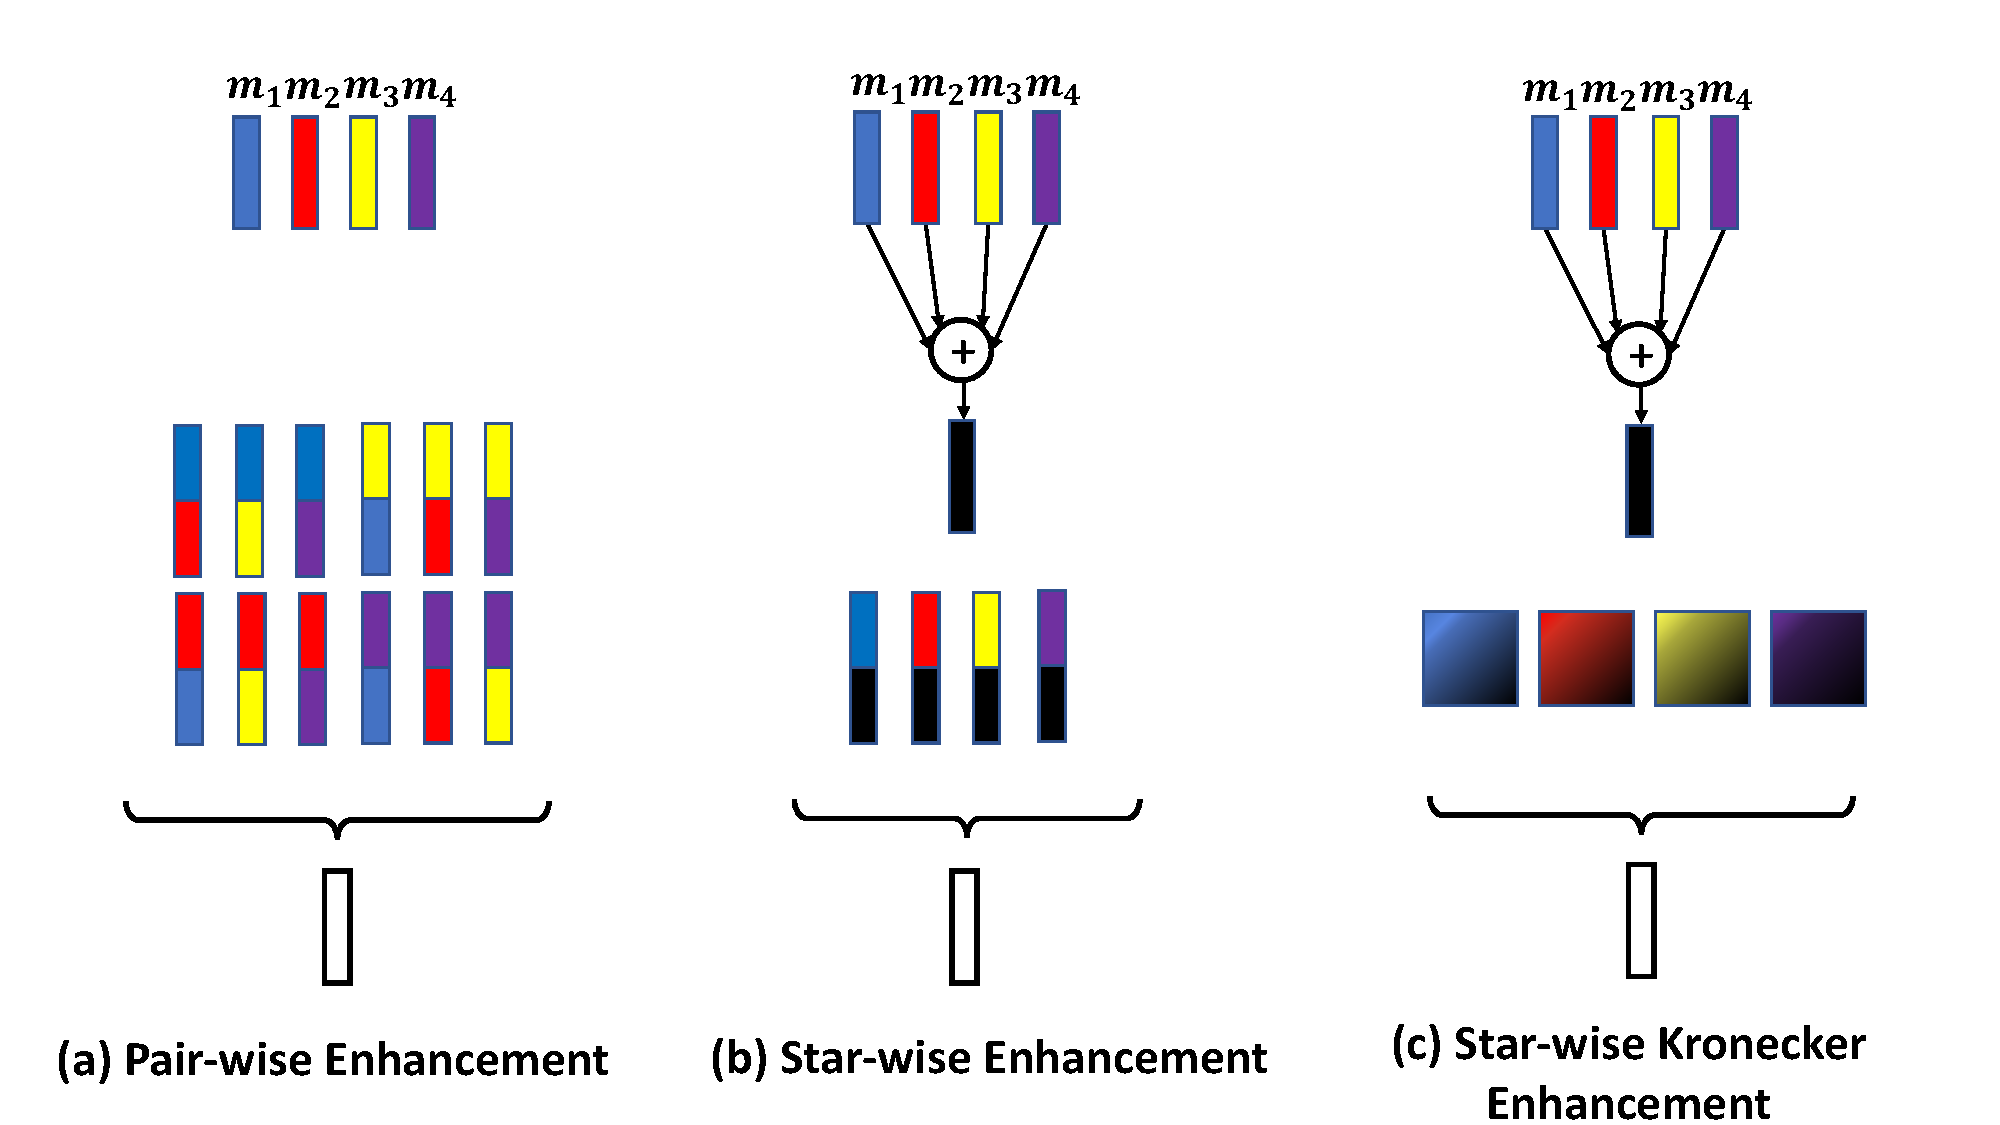
\includegraphics[scale=0.25]{filter_figure.pdf}
\end{center}
%\setlength{\abovecaptionskip}{-5pt}
%  \setlength{\belowcaptionskip}{-5pt}
\vspace{-4mm}
   \caption{Architecture} 
\label{fig_archi}
\vspace{-5mm}
\end{figure}
\subsubsection{The Filter Generator:} The objective of the filter generator, $f_\phi$, is to exploit the signal provided by the  neighbourhood $\mathcal{N}_i$ to produce a filter that maximally enhances the discriminative information for a given task. Intuitively, enhancement can be achieved through resolving ambiguity within a signal via reference to cues from its neighbours. It follows that to achieve this objective, the functional form of the generator should allow it to reason about the relationship between the contextual signal of the neighbourhood and the signal to be filtered.  To design such a generator, we draw inspiration from the Relation Network (RN) \cite{santoro2017simple}, and consider the following functional form for the filter generator:
\begin{equation} \label{pairwise} 
 f_\phi (\{\bm_j: j \in \mathcal{N}_i\}) = h_\phi (\sum_{j\neq i} g_\theta (m_i,m_j)),
\end{equation}
where functions $h_\phi$ and $g_\theta$ are used to model the pairwise relationship between signal $m_i$ and  $m_j$. More specifically, $g_\theta$ aims to aggregate structure information from each neighbour and $h_\phi$ combines the information from different sources. It dictates that the filter aims to learn and infer the existence and implication of all pair-wise signal relations within its filter field. 


However, the fully pairwise formulation typically contains many connections and parameters, which thus naturally brings redundancy in the connections, and also makes the network optimisation more difficult, particularly in the presence of limited training data. In order to substantially reduce the computational overhead of large fully-connected graphs, we modify the functional form described above.  Concretely, we propose to prune the set of relational pairs to the star topology imposed via Eqn.~\ref{star}.


% an intuition solution should be reducing the filter receptive field. However in various machine learning tasks, learning deep representations capturing both local and global receptive fields is important for the model performance [37, 35]. To maintain a large filter receptive field while utilising much fewer parameters than the fully-connected setting,  

\begin{equation} \label{star} 
 f_\phi (\{\bm_j: j \in \mathcal{N}_i\}) = h_\phi (g_\theta (m_i,\sum_{j} m_j)),
\end{equation}

This function combines a single pooling operator over all neighbours within the filter field to first obtain the context vector representation. Then for each signal, only relations between the input with the context vector are directly inferred. Such an approach encourages greater generalisation for computing relations, since $g_\theta$ is encouraged to not over-fit to the features of any particular signal. In contrast to the quadratic computational complexity pairwise topology implied by Eqn.~\ref{eqn:cmf}, the cost of a forward pass through the star-topology scales linearly with the number of inputs (see Fig.~\ref{fig_archi} centre). It is also worth noting that the star topology the summation in Eqn.~\ref{star} also ensures that the filter is invariant to the order of objects in the input signal. This invariance ensures that the filter output contains information that is generally representative of the relations that exist in the signal set.
 
While Eqn.~\ref{star} brings computational efficiency, it comes at a cost.  In essence, by exchanging the ordering of the summation over signals and $g_\theta$, the functional form of the filter generator no longer forms a natural for the pairwise interactions amongst the inputs.  In order to preserve the effective modelling capacity of the generator, whilst at the same time maintaining its attractive linear scaling, we therefore look to \textit{approximate} the the set of interactions directly in feature space.  We perform this approximation via a tensor product between the context vector and the incoming filter.  Intuitively, the tensor product offers a simple mechanism for  modelling interactions between feature sets \cite{long2017deep}, since each feature in the tensor product space corresponds to the product of a pair of features in the original feature set. Prior work has shown that this approximation of the statistics of the joint feature representations between two features \cite{song2013robust} is reasonable, given appropriate sample sizes. In more detail, we perform the tensor product between the $i^{(th)}$ modality signal $m_i$ and the context vector $\sum_{j} m_j$ when forming the input to function $g_\theta$, providing additional information in comparison to direct feature concatenation.  However, for even moderately sized input signals, the use a tensor product $m_i \otimes \sum_{j} m_j$ would be prohibitively expensive in both computation and memory.  We therefore opt to first project both operands of the tensor product to a lower dimension via a learnable linear projection $g_\theta$, prior to performing the tensor product:

\begin{equation} \label{star} 
 f_\phi (\{\bm_j: j \in \mathcal{N}_i\}) = h_\phi (g_\theta (m_i) \otimes g_\theta (\sum_{j} m_j)),
\end{equation}

% @Yang, I don't understand what this means.... :)
% Another tight approximation of the original  Eq ~(\ref{pairwise}) is calculating the tensor product between each single signal with the context vector. Assuming we have two vector spaces $V$ and $U$, their tensor product $V \otimes U$ intuitively is the idea "for each vector $v \in V$ ", attach it the entire vector space $U$.
% To obtain  $V \otimes U$, we start from the product space $U \times V$ and consider the free abelian group oover it denoted by $\mathcal{F}(U \times V)$. Given this larger space, that admits scalar products of ordered pairs, we we set up equicalence relations of the form $(av, u) a(v, u) (v,au) $ with $u \in U$, $v \in V$ and $a in \mathcal{F}$(a field) so that we identify points in the product space that yield multi-linear relationships in the quotient space generated by these relationships.

% \begin{itemize}

%     \item Pairwise CE.  Used in prior work.  Inspired by the Relation Network \cite{santoro2017simple}
%     \item The star topology
%     \item The Kronecker product approximation to the joint distribution.
%     % \item The triplet topology
% \end{itemize}
\subsubsection{Application Function:} Finally, we consider the choice of application function $a_\theta$.  While many choices are possible here, we follow prior work  successful designs of attention mechanism for feature enhancement (e.g. \cite{dauphin2017language,hu2019squeeze}) which apply a sigmoid operator over the generated filter to produce a $[0, 1]$-normalised mask. This mask is then multiplied element-wise back through the original signal.

% \textbf{Relationship to Attention}: One interpretation of Cross-Modal Enhancement is as an attention mechanism operating between the incoming signals.    {Maybe we want to talk about the relationship with dynamic filter, Message passing neural networks, attention mechanisms, etc.}



% As the number of inputs grows, it may be desirable to impose sparsity on the inclusion graph 

% In the absence of prior knowledge indicating that the a sparse graph should be used, a natural choice for the filtering neighbourhood in 

% We first assume access to a collection of modality-specific feature extractors $\{ \Phi_m \}_{m \in \mathcal{M}}$.  These may operate at either the video-level, or in the case of visual models, at the frame-level.  For example, one such frame-level feature extractor operating on the visual modality could be a convolutional neural network whose parameters have been optimised for the task for image classification.  This model therefore transforms the raw pixel data present in each frame of a video into a single embedding.  We next assume access to a corresponding family of temporal aggregation functions $\{ T_m \}_{m \in \mathcal{M}}$, which transform, for each feature extractor, its outputs into a fixed size representation.  A temporal aggregation function may be heavily parameterised, or simply comprise a pooling operation such as max or sum pooling. 

% Given the above, our goal is to transform the temporally aggregated modality-specific feature extractors $\{T_m(\Phi_m(\mathbf{v})): m \in \mathcal{M}\}$ of the source video that compactly represents the content within it that is relevant for a given task.  There are many ways 

% We reason via a lightweight attention mechanims.  The core idea (CE).

% \subsection{Extension to higher order interactions}



% \subsection{AHOI: An Efficient Approximation to higher-order reasoning}
\\
The general nature of the CME design described above allow for its direct integration into architectures for video understanding.  We its investigate its application in two representative tasks: text-video retrieval and action recognition, described next.

\subsection{Text-Video Retrieval Model}

The task of text-video retrieval requires a system to rank a collection of videos according to how well they match a given text query.  Joint video-text embeddings (which seek to map videos and text descriptions into a common space such that matching video and text pairs are close together) form an attractive model for tackling this problem, since they readily allow for efficient indexing: compact video embeddings can be pre-computed and stored offline such that the test time query reduces to simple distance computation between embeddings.

To assess the proposed CME approach, we adopt as a backbone the MoEE/CENet joint text-video embedding architecture proposed by \cite{miech2018learning} and extended more recently by \cite{liu2019use}.  In particular, the CENet architecture represents the state-of-the-art on several popular retrieval benchmarks.  Moreover, it utilises a particular form of \textit{pairwise} filtering to combine different signals of different modalities, making it an ideal starting point for our investigations.   We first briefly summarise the model, then describe the integration of CME as a component of the architecture.

The MoEE/CENet architecture comprises two core elements: a video encoder and a text encoder, which are learned to map videos and text into a common space.  CENet derives its strong retrieval performance by composing together the embeddings of a diverse collection of ``experts'': these are machine perception models which have been pretrained for related tasks, but not directly for retrieval.  In particular, they use deep neural networks pretrained for classification on the ImageNet dataset~\cite{deng2009imagenet}, scene recognition on the Places dataset \cite{zhou2017places}, action recognition models pretrained on Kinetics~\cite{}


\subsection{Action Recognition Model}

\begin{figure*}
    \centering
    \includegraphics[width=\textwidth,height=2in]{example-image-a}
    \caption{\textbf{The family of filter generation functions considered in this work}.}
    \label{fig:reasoning}
\end{figure*}
\section{Experiments}


In this section, we first evaluate the proposed CMF module on two tasks: text-video retrieval and very-large scale action recognition. Then we present an ablation study to explore how the performance of the proposed approach is affected by different CMF designs. 

% In this section, We first provide the description of datasets, implementation details and evaluation metric used in two tasks. Then We evaluate the proposed CMF approach on four benchmarks for video retrieval and a large scale action recognition benchmark. Finally we present an ablation study to explore how the performance of the proposed approach is affected by different CMF designs. 



\subsection{Video Retrieval}

\subsubsection{Dataset and Implementation Details}

We perform experiments on four video datasets:  MSR-VTT~\cite{xu2016msr}, LSMDC~\cite{rohrbach2015dataset}, DiDeMo~\cite{anne2017localizing} and ActivityNet-captions~\cite{krishna2017dense}, covering a challenging set of domains which include videos from YouTube, personal collections and movies. 

We begin by evaluating the module on standard text-video retrieval benchmarks.  \samsays{TODO: Add detailed dataset descriptions and evaluation protocols}


\paragraph{ActivityNet-captions:} \cite{krishna2017dense} comprises a collection of 20k videos sourced from YouTube.  Each video is accompanied by a descriptive sentences, numbering 100k in total.  For fair comparison, we adopt the retrieval evaluations and protocols used in prior work \cite{zhang2018cross,liu2019use}, training up to 15 epochs on the training partition (10,009 videos in total) and evaluating on the larger \texttt{val1} (4,917 videos in total).  We report performance in Tab.~\ref{table:activity-net}.


\begin{table*}[h]
% \captionsetup{font=footnotesize}
\centering 
\footnotesize 
\setlength{\tabcolsep}{5pt}
\begin{tabular}{l | c c c c c | c c c c c} 
\hline \hline 
\multicolumn{1}{c}{} & 
\multicolumn{5}{c}{Text $\implies$ Video} & \multicolumn{5}{c}{Video $\implies$ Text} \\
Method & R$@$1 & R$@$5 & R$@$50 & MdR & MnR & R$@$1 & R$@$5 & R$@$50 & MdR & MnR \\ 
\hline 
LSTM-YT & 0.0 & 4.0 & 24.0 & 102 & - & 0.0 & 7.0 & 38.0  & 98 & - \\
NOCTXT & 5.0 & 14.0 & 32.0 & 78 & - & 7.0 & 18.0 & 45.0 & 56 & - \\

DENSE & 14.0 & 32.0 & 65.0 & 34 & - & 18.0 & 36.0 & 74.0 & 32 \\
HSE(4SEGS) & 20.5 & 49.3 & - & - & - & 18.7 & 48.1 & - & - \\
FSE & $\prepad 18.2_{\pm0.2}$ & $\prepad 44.8_{\pm0.4}$ & $\prepad {89.1}_{\pm 0.3}$ & $7$ & - & $\prepad {16.7}_{\pm0.8}$ & $\prepad {43.1}_{\pm1.1}$ & $\prepad 88.4_{\pm0.3}$ & $7$ &  - \\
CE & $\prepad 27.3_{\pm0.7}$ & $\prepad 61.1_{\pm1.0}$ & $\prepad 94.4_{\pm0.1}$ & $\prepadmini 4_{\pm0}$ & $\prepad 15.4_{\pm0.9}$ 
& $\prepad 27.9_{\pm0.6}$ & $\prepad 61.6_{\pm0.4}$ & $\prepad 95.0_{\pm0.2}$ & $\prepadmini 3.3_{\pm0.6}$ & $\prepad 14.5_{\pm0.8}$ \\
\hline
% CMF-pairwise & $\prepad 31.6_{\pm0.3}$ & $\prepad 67.2_{\pm0.2}$ & $\prepad 97.0_{\pm0.2}$ & $\prepad 3.0_{\pm0.0}$ & $\prepad 9.9_{\pm0.1}$ & $\prepad 32.0_{\pm0.4}$ & $\prepad 68.9_{\pm1.1}$ & $\prepad 97.1_{\pm0.3}$ & $\prepad 3.0_{\pm0.0}$ & $\prepad 9.5_{\pm0.4}$ \\
% CMF-pairwise-star & $\prepad 31.7_{\pm0.5}$ & $\prepad 66.9_{\pm0.6}$ & $\prepad 96.7_{\pm0.3}$ & $\prepad 3.0_{\pm0.0}$ & $\prepad 10.0_{\pm0.3}$ & $\prepad 32.7_{\pm0.4}$ & $\prepad 69.2_{\pm0.8}$ & $\prepad 96.9_{\pm0.1}$ & $\prepad 3.0_{\pm0.0}$ & $\prepad 9.4_{\pm0.3}$ \\
CMF-pairwise-star-tensor & $\prepad 32.3_{\pm0.3}$ & $\prepad 67.6_{\pm0.3}$ & $\prepad 97.2_{\pm0.1}$ & $\prepad 3.0_{\pm0.0}$ & $\prepad 9.50_{\pm0.2}$ & $\prepad 33.5_{\pm0.7}$ & $\prepad 69.2_{\pm1.2}$ & $\prepad 97.4_{\pm0.1}$ & $\prepad 3.0_{\pm0.0}$ & $\prepad 8.9_{\pm0.6}$ \\
% CMF-triplet & $\prepad 30.5_{\pm0.2}$ & $\prepad 66.5_{\pm0.7}$ & $\prepad 96.8_{\pm0.1}$ & $\prepad 3.0_{\pm0.0}$ & $\prepad 9.8_{\pm0.2}$ & $\prepad 32.0_{\pm1.4}$ & $\prepad 67.5_{\pm0.8}$ & $\prepad 96.8_{\pm0.4}$ & $\prepad 3.0_{\pm0.0}$ & $\prepad 9.4_{\pm0.6}$ \\
% % CMF-pairwise-star-random & $\prepad 27.4_{\pm0.7}$ & $\prepad 62.6_{\pm1.4}$ & $\prepad 96.1_{\pm0.1}$ & $\prepad 3.0_{\pm0.0}$ & $\prepad 11.3_{\pm0.3}$ & $\prepad 29.6_{\pm0.6}$ & $\prepad 65.5_{\pm1.0}$ & $\prepad 96.8_{\pm0.1}$ & $\prepad 3.0_{\pm0.0}$ & $\prepad 10.2_{\pm0.2}$ \\
% CMF-pairwise-star-specific & $\prepad 31.1_{\pm0.7}$ & $\prepad 65.9_{\pm1.4}$ & $\prepad 96.8_{\pm0.1}$ & $\prepad 3.0_{\pm0.0}$ & $\prepad 10.1_{\pm0.3}$ & $\prepad 31.9_{\pm0.6}$ & $\prepad 67.6_{\pm1.0}$ & $\prepad 96.9_{\pm0.1}$ & $\prepad 3.0_{\pm0.0}$ & $\prepad 9.5_{\pm0.2}$ \\

\hline \hline
\end{tabular}
% \vspace{0.3cm}
\caption{\color{red}Comparison of paragraph-video retrieval methods trained with video-level information on the ActivityNet-captions dataset (val1 test-split). For reference: LSTM-YT~\cite{venugopalan2015sequence} (\cite{zhang2018cross}), NOCTXT~\cite{venugopalan2014translating} (\cite{zhang2018cross}), HSE(4SEGS)~\cite{zhang2018cross}, DENSE~\cite{krishna2017dense}, FSE~\cite{zhang2018cross} \color{black}}
\label{table:activity-net} 
\end{table*}

\paragraph{DiDeMo:} \cite{anne2017localizing} consists of a set of personal videos, captured in a diverse array of visual settings (10,464 videos in total).  We follow prior work on \textit{video-level} text-video retrieval (we do not make use of timestamp information during training or testing).  We compare to competing methods in Tab.~\ref{table:DiDeMo}.  \samsays{We may need to report numbers on the DiDeMo val set for a fair comparison with CE.}


\begin{table*}[h!]
\centering 
\footnotesize 
\setlength{\tabcolsep}{2pt}
\begin{tabular}{l | c c c c c | c c c c c} 
\hline \hline
\multicolumn{1}{c}{} & 
\multicolumn{5}{c}{Text $\implies$ Video} & \multicolumn{5}{c}{Video $\implies$ Text} \\
Method & R$@$1 & R$@$5 & R$@$50 & MdR & MnR & R$@$1 & R$@$5 & R$@$50 & MdR & MnR \\ 
\hline 
S2VT  & 11.9 & 33.6 & 76.5 & 13 & - & 13.2 & 33.6 & 76.5 & 15 & - \\
FSE & $\prepad 13.9_{\pm0.7}$ & $\prepad 36_{\pm0.8}$ & $\prepad {78.9}_{\pm 1.6}$ & $11$ & - & $\prepad {13.1}_{\pm0.5}$ & $\prepad {33.9}_{\pm0.4}$ & $\prepad 78.0_{\pm0.8}$ & $12$ &  - \\
CE & $\prepad 22.6_{\pm0.5}$ & $\prepad 51.1_{\pm1.0}$ & $\prepad 87.3_{\pm0.3}$ & $\hspace{1em} 5_{\pm0}$ & $\prepad 27.4_{\pm1.1}$ & $\prepad 22.5_{\pm1.3}$ & $\prepad 52.3_{\pm0.8}$ & $\prepad 89.2_{\pm0.8}$ & $\hspace{1em} 5_{\pm0}$ & $\prepad 23.2_{\pm1.1}$ \\
\hline
% CMF-pairwise-star & $\prepad 25.0_{\pm0.7}$ & $\prepad 54.8_{\pm0.4}$ & $\prepad 91.0_{\pm1.3}$ & $\prepad 4.3_{\pm0.6}$ & $\prepad 17.3_{\pm0.5}$ & $\prepad 24.4_{\pm1.0}$ & $\prepad 55.2_{\pm1.4}$ & $\prepad 93.7_{\pm0.4}$ & $\prepad 4.0_{\pm0.0}$ & $\prepad 14.0_{\pm0.4}$ \\
% CMF-pairwise-noMOE & $\prepad 25.4_{\pm1.3}$ & $\prepad 54.5_{\pm0.4}$ & $\prepad 91.8_{\pm0.3}$ & $\prepad 4.3_{\pm0.6}$ & $\prepad 17.1_{\pm0.3}$ & $\prepad 25.1_{\pm0.8}$ & $\prepad 56.1_{\pm1.0}$ & $\prepad 93.4_{\pm0.8}$ & $\prepad 4.0_{\pm0.0}$ & $\prepad 14.0_{\pm0.5}$ \\
CMF-pairwise-star-tensor & $\prepad 25.4_{\pm0.4}$ & $\prepad 54.2_{\pm0.3}$ & $\prepad 91.6_{\pm0.7}$ & $\prepad 4.7_{\pm0.6}$ & $\prepad 17.3_{\pm0.9}$ & $\prepad 25.4_{\pm1.2}$ & $\prepad 56.0_{\pm0.4}$ & $\prepad 93.8_{\pm1.1}$ & $\prepad 4.0_{\pm0.0}$ & $\prepad 14.0_{\pm0.6}$ \\
% CMF-triplet & $\prepad 24.6_{\pm0.7}$ & $\prepad 55.0_{\pm0.9}$ & $\prepad 91.7_{\pm0.6}$ & $\prepad 4.3_{\pm0.6}$ & $\prepad 16.7_{\pm0.8}$ & $\prepad 26.1_{\pm0.6}$ & $\prepad 56.0_{\pm2.0}$ & $\prepad 93.6_{\pm0.8}$ & $\prepad 4.3_{\pm0.6}$ & $\prepad 13.7_{\pm0.8}$ \\
% CMF-pairwise-star-avgmax & $\prepad 24.2_{\pm0.5}$ & $\prepad 55.0_{\pm0.6}$ & $\prepad 91.8_{\pm0.4}$ & $\prepad 4.3_{\pm0.6}$ & $\prepad 16.8_{\pm0.4}$ & $\prepad 25.6_{\pm0.9}$ & $\prepad 55.5_{\pm1.4}$ & $\prepad 93.8_{\pm0.4}$ & $\prepad 4.3_{\pm0.6}$ & $\prepad 14.1_{\pm0.4}$ \\
% CMF-pairwise-star-random & $\prepad 15.9_{\pm8.5}$ & $\prepad 37.5_{\pm12.8}$ & $\prepad 80.5_{\pm9.3}$ & $\prepad 11.3_{\pm5.5}$ & $\prepad 36.5_{\pm15.2}$ & $\prepad 15.1_{\pm10.0}$ & $\prepad 36.6_{\pm15.2}$ & $\prepad 80.0_{\pm11.1}$ & $\prepad 12.3_{\pm7.2}$ & $\prepad 38.1_{\pm20.7}$ \\

\hline \hline
\end{tabular}
\caption{\color{red}Paragraph-video retrieval comparison of  methods trained with video-level information on the DiDeMo benchmark. For reference: SV2T~\cite{venugopalan2014translating} (\cite{zhang2018cross}), FSE~\cite{zhang2018cross}\color{black}}
\label{table:DiDeMo} 
\end{table*}

\paragraph{MSR-VTT:} \cite{xu2016msr} We report results in Tab.~\ref{table:MSRVTT}. 

\begin{table*}[t]
\centering 
\footnotesize 
% \setlength{\tabcolsep}{2pt}
\begin{tabular}{l | c | c c c c c |@{\hskip -0.2cm}c@{\hskip -0.35cm}c@{\hskip -0.35cm}c@{\hskip -0.1cm}c@{\hskip -0.2cm}c} 
\hline \hline
\multicolumn{2}{c}{} & 
\multicolumn{5}{c}{Text $\implies$ Video} & \multicolumn{5}{c}{Video $\implies$ Text} \\
Method  & R$@$1 & R$@$5 & R$@$10 & MdR & MnR & R$@$1 & R$@$5 & R$@$10 & MdR & MnR \\ 
\hline 
% \textbf{HOI}  & 1k-B & $\prepad \mathbf{00.0}_{\pm0.0}$  & $\prepad \mathbf{00.0}_{\pm0.0}$  &  $\prepad \mathbf{00.0}_{\pm0.0}$  &  $\prepadmini \mathbf{0}_{\pm0}$ & $\prepad \mathbf{0.0}_{\pm0.0}$ & $\prepad \mathbf{00.0}_{\pm0.0}$ & $\prepad \mathbf{00.0}_{\pm0.0}$  & $\prepad \mathbf{00.0}_{\pm0.0}$  &  $\prepadmini \mathbf{0}_{\pm0}$ & $\prepad \mathbf{0.0}_{\pm0.0}$ \\
% \textbf{AHOI}  & 1k-B & $\prepad \mathbf{00.0}_{\pm0.0}$  & $\prepad \mathbf{00.0}_{\pm0.0}$  &  $\prepad \mathbf{00.0}_{\pm0.0}$  &  $\prepadmini \mathbf{0}_{\pm0}$ & $\prepad \mathbf{0.0}_{\pm0.0}$ & $\prepad \mathbf{00.0}_{\pm0.0}$ & $\prepad \mathbf{00.0}_{\pm0.0}$  & $\prepad \mathbf{00.0}_{\pm0.0}$  &  $\prepadmini \mathbf{0}_{\pm0}$ & $\prepad \mathbf{0.0}_{\pm0.0}$ \\
\hline 
VSE  & 5.0 & 16.4 & 24.6 & 47 & 215.1 & 7.7 & 20.3 & 31.2 & 28 & 185.8\\
VSE++ & 5.7 & 17.1 & 24.8 & 65 & 300.8 & 10.2 & 25.4 & 35.1 & 25 & 228.1 \\
Mithun et al. &  7.0 & 20.9 & 29.7 & 38 & 213.8  & 12.5 & 32.1 & 42.4 & 16 & 134.0 \\
W2VV & 6.1 & 18.7 & 27.5 & 45 & - &  11.8 & 28.9 & 39.1 & 21 & -  \\  
Dual Encoding & 7.7 & 22.0 & 31.8 & 32 & - &  13.0 & 30.8 & 43.3 & 15 & - \\
\textbf{CE}  & $\prepad \mathbf{22.5}_{\pm0.1}$ & $\prepad \mathbf{52.1}_{\pm0.2}$ & $\prepad \mathbf{65.5}_{\pm0.1}$ & $\prepadmini \mathbf{5}_{\pm0}$ & $\quad \mathbf{22.5}_{\pm0.1}$ & $\quad \mathbf{34.4}_{\pm0.4}$ & $\prepad \mathbf{64.6}_{\pm0.3}$ & $\prepad \mathbf{77.0}_{\pm0.4}$ & $\prepadmini \mathbf{3}_{\pm0}$ & $\prepad \mathbf{13.2}_{\pm0.6}$ \\
CME-pairwise & $\prepad 23.2_{\pm0.2}$ & $\prepad 54.7_{\pm0.3}$ & $\prepad 68.8_{\pm0.3}$ & $\prepad 4.7_{\pm0.6}$ & $\prepad 17.1_{\pm0.1}$ & $\prepad 32.5_{\pm0.4}$ & $\prepad 67.5_{\pm0.4}$ & $\prepad 80.1_{\pm0.2}$ & $\prepad 3.0_{\pm0.0}$ & $\prepad 9.7_{\pm0.4}$ \\
CME-pairwise-star & $\prepad 22.9_{\pm0.3}$ & $\prepad 54.3_{\pm0.3}$ & $\prepad 68.6_{\pm0.3}$ & $\prepad 5.0_{\pm0.0}$ & $\prepad 17.2_{\pm0.1}$ & $\prepad 33.4_{\pm0.5}$ & $\prepad 67.9_{\pm0.2}$ & $\prepad 80.1_{\pm0.6}$ & $\prepad 3.0_{\pm0.0}$ & $\prepad 9.6_{\pm0.3}$ \\
CMF-pairwise-star-tensor & $\prepad 23.0_{\pm0.1}$ & $\prepad 54.5_{\pm0.3}$ & $\prepad 68.6_{\pm0.3}$ & $\prepad 4.7_{\pm0.6}$ & $\prepad 17.2_{\pm0.2}$ & $\prepad 33.2_{\pm0.6}$ & $\prepad 68.2_{\pm1.1}$ & $\prepad 80.6_{\pm0.7}$ & $\prepad 2.8_{\pm0.3}$ & $\prepad 9.5_{\pm0.2}$ \\
CME-pairwise-star-specific & $\prepad 22.9_{\pm0.1}$ & $\prepad 54.4_{\pm0.4}$ & $\prepad 68.8_{\pm0.1}$ & $\prepad 4.7_{\pm0.6}$ & $\prepad 17.1_{\pm0.1}$ & $\prepad 33.6_{\pm1.1}$ & $\prepad 67.4_{\pm0.3}$ & $\prepad 79.7_{\pm0.4}$ & $\prepad 3.0_{\pm0.0}$ & $\prepad 9.8_{\pm0.4}$ \\
% \textbf{HOI}  & Full & $\prepad \mathbf{00.0}_{\pm0.0}$  & $\prepad \mathbf{00.0}_{\pm0.0}$  &  $\prepad \mathbf{00.0}_{\pm0.0}$  &  $\prepadmini \mathbf{0}_{\pm0}$ & $\prepad \mathbf{0.0}_{\pm0.0}$ & $\prepad \mathbf{00.0}_{\pm0.0}$ & $\prepad \mathbf{00.0}_{\pm0.0}$  & $\prepad \mathbf{00.0}_{\pm0.0}$  &  $\prepadmini \mathbf{0}_{\pm0}$ & $\prepad \mathbf{0.0}_{\pm0.0}$ \\
% \textbf{AHOI}  & Full & $\prepad \mathbf{00.0}_{\pm0.0}$  & $\prepad \mathbf{00.0}_{\pm0.0}$  &  $\prepad \mathbf{00.0}_{\pm0.0}$  &  $\prepadmini \mathbf{0}_{\pm0}$ & $\prepad \mathbf{0.0}_{\pm0.0}$ & $\prepad \mathbf{00.0}_{\pm0.0}$ & $\prepad \mathbf{00.0}_{\pm0.0}$  & $\prepad \mathbf{00.0}_{\pm0.0}$  &  $\prepadmini \mathbf{0}_{\pm0}$ & $\prepad \mathbf{0.0}_{\pm0.0}$ \\
\hline \hline
\end{tabular}
\vspace{0.2cm}
\caption{\color{red}Retrieval using sentences and videos on the MSR-VTT dataset. R$@$k denotes recall$@$k (higher is better), MdR and MnR denote median rank and mean rank resp. (lower is better). 1k-A and 1k-B denote test sets of 1000 randomly sampled text-video pairs used by~\cite{yu2018joint} and~\cite{miech2018learning} resp.  We report standard deviations from three randomly seeded runs.  $\ddagger$~Updated code-base released by Miech et al.~\cite{miech2018learning} which achieves stronger results. For reference: JSFusion~\cite{yu2018joint}, MoEE~\cite{miech2018learning}, VSE~\cite{mithun2018learning}, VSE++ \cite{mithun2018learning}, W2VV~\cite{dong2018predicting}, Dual Encoding~\cite{dong2018dual} \color{black}}
\label{table:MSRVTT} 
\end{table*}

\normalsize

\paragraph{LSMDC:} \cite{rohrbach2015dataset}.  We report results in Tab.~\ref{table:LSMDC-MSVD} (left)

\begin{table*}[ht]
\centering 
\begin{minipage}{0.45\linewidth}
\footnotesize
\setlength{\tabcolsep}{5pt}
\hspace{-5em}
\begin{tabular}{l | c c c c }
\hline \hline
\multicolumn{1}{c}{} & 
\multicolumn{4}{c}{Text $\implies$ Video} \\
Method & R$@$1 & R$@$5 & R$@$10 & MdR  \\ 
\hline 
Yu et al.$\dagger$ &3.6 & 14.7 & 23.9 & 50 \\
CCA  &7.5 & 21.7 & 31.0 & 33  \\
JSFusion $\ddagger$  & 9.1 & 21.2 & 34.1 & 36  \\
MoEE &  11.6 & 28.0 & 37.6 & 22   \\
$\text{MoEE}_\text{COCO}$ &  12.7 & 28.9 & 39.6 & 21   \\
\textbf{CE}  & $\prepad 12.6_{\pm0.8}$ & $\prepad 31.0_{\pm0.6}$ & $\prepad 40.3_{\pm0.5}$ & $\hspace{0.8em} 19_{\pm0}$  \\
\hline
No-CMF & \prepad 15.0_{\pm0.2} & \prepad 32.5_{\pm0.6} & \prepad 42.9_{\pm0.8} & \prepad 16.0_{\pm0.0} \\
CMF-pairwise & \prepad 17.2_{\pm0.4} & \prepad 37.6_{\pm0.6} & \prepad 48.9_{\pm0.7} & \prepad 11.3_{\pm0.6} \\
CMF-pairwise-star & \prepad 16.7_{\pm0.1} & \prepad 37.5_{\pm1.0} & \prepad 48.3_{\pm0.7} & \prepad 11.3_{\pm0.6} \\
CMF-triplet & \prepad 17.8_{\pm1.2} & \prepad 37.7_{\pm1.4} & \prepad 47.9_{\pm1.2} & \prepad 12.0_{\pm1.0} \\
CMF-pairwise-star+ & \prepad 17.9_{\pm1.2} & \prepad 38.4_{\pm0.5} & \prepad 48.6_{\pm0.9} & \prepad 11.3_{\pm0.6} \\
\hline \hline
\end{tabular}
\end{minipage}
\begin{minipage}{0.4\linewidth}
\centering 
\footnotesize
% \setlength{\tabcolsep}{4pt}
\begin{tabular}{l | c c c c c } 
\hline \hline
\multicolumn{1}{c}{} & 
\multicolumn{5}{c}{Text $\implies$ Video}  \\
Method & R$@$1 & R$@$5 & R$@$10 & MdR & MnR  \\ 
\hline 
CCA  & - & - & - & - & 245.3  \\
JMDV  & - & - & - & - & 236.3  \\
VSE  & 12.3 & 30.1 & 42.3 & 14 & 57.7 \\
VSE++ & 15.4 & 39.6 & 53.0 & 9 & 43.8 \\
Multi. Cues  & 20.3 & 47.8 & 61.1 & $\textbf{6}$ & 28.3 \\

CE  & $\prepad 20.9_{\pm0.5}$ & $\prepad 49.7_{\pm0.4}$ & $\prepad 63.8_{\pm0.4}$ & $\prepad 5.7_{\pm0.6}$ & $\prepad 19.5_{\pm0.9}$ \\
\hline
% (No CMF) & \prepad 15.0_{\pm0.2} & \prepad 32.5_{\pm0.6} & \prepad 42.9_{\pm0.8} & \prepad 69.2_{\pm0.8} & \prepad 16.0_{\pm0.0} & \prepad 56.8_{\pm0.2} & \prepad 19.0_{\pm0.2} & \prepad 39.5_{\pm0.9} & \prepad 50.0_{\pm1.1} & \prepad 77.9_{\pm0.8} & \prepad 10.7_{\pm0.6} & \prepad 35.1_{\pm0.7}

% CE & $\prepad 00.0_{\pm0.0}$ & $\prepad 00.0_{\pm0.0}$ & $\prepad 00.0_{\pm0.0}$ & $\prepad 0.0_{\pm0.0}$ & $\prepad 00.0_{\pm0.0}$ \\
% AHOI  & $\prepad 00.0_{\pm0.0}$ & $\prepad 00.0_{\pm0.0}$ & $\prepad 00.0_{\pm0.0}$ & $\prepad 0.0_{\pm0.0}$ & $\prepad 00.0_{\pm0.0}$ \\
\hline
CMF & (still cooking) & & & \\
\hline \hline
\end{tabular}
\end{minipage}
\vspace{0.2cm}
\caption{\color{red}Text-to-Video retrieval results on the LSMDC dataset (left) and the MSVD dataset (right). $\dagger,\ddagger$ denote the winners of the 2016 and 2017 LSMDC challenges, respectively. For reference: MoEE and CCA~\cite{miech2018learning}, JSFusion~\cite{yu2018joint}, JMDV, CCA (right)~\cite{xu2015jointly}, Yu et al.~\cite{yu2016video}, VSE \cite{kiros2014unifying} (\cite{mithun2018learning}), VSE++ \cite{faghri2017vse} (\cite{mithun2018learning}), Multi. Cues \cite{mithun2018learning}  \color{black}}
\label{table:LSMDC-MSVD} 
\end{table*}


\paragraph{MSVD:} \cite{chen2011collecting}  We report results in Tab.~\ref{table:LSMDC-MSVD} (right)

\subsection{Action Recognition}

\paragraph{Multi-Moments-in-Time:} This dataset is a recently released very-large scale collection of short videos for action recognition.  The Multi-Moments-in-Time dataset contains 313 classes, 1025862 training videos and 10000 validation videos \cite{monfortmoments}.

\subsection{Ablation Study: Module Design}

In this section, we assess the contribution of the proposed HOI module.  To do so, we conduct further experiments on the MSR-VTT dataset as well as the Mult-Moments-in-Time dataset.
\begin{table*}[h]
% \captionsetup{font=footnotesize}
\centering 
\footnotesize 
\setlength{\tabcolsep}{5pt}
\begin{tabular}{l | c c c c c | c c c c c} 
\hline \hline 
\multicolumn{1}{c}{} & 
\multicolumn{5}{c}{Text $\implies$ Video} & \multicolumn{5}{c}{Video $\implies$ Text} \\
Method & R$@$1 & R$@$5 & R$@$50 & MdR & MnR & R$@$1 & R$@$5 & R$@$50 & MdR & MnR \\ 

\hline
CMF-pairwise & $\prepad 31.6_{\pm0.3}$ & $\prepad 67.2_{\pm0.2}$ & $\prepad 97.0_{\pm0.2}$ & $\prepad 3.0_{\pm0.0}$ & $\prepad 9.9_{\pm0.1}$ & $\prepad 32.0_{\pm0.4}$ & $\prepad 68.9_{\pm1.1}$ & $\prepad 97.1_{\pm0.3}$ & $\prepad 3.0_{\pm0.0}$ & $\prepad 9.5_{\pm0.4}$ \\
CMF-pairwise-star & $\prepad 31.7_{\pm0.5}$ & $\prepad 66.9_{\pm0.6}$ & $\prepad 96.7_{\pm0.3}$ & $\prepad 3.0_{\pm0.0}$ & $\prepad 10.0_{\pm0.3}$ & $\prepad 32.7_{\pm0.4}$ & $\prepad 69.2_{\pm0.8}$ & $\prepad 96.9_{\pm0.1}$ & $\prepad 3.0_{\pm0.0}$ & $\prepad 9.4_{\pm0.3}$ \\
CMF-pairwise-star-tensor & $\prepad 32.3_{\pm0.3}$ & $\prepad 67.6_{\pm0.3}$ & $\prepad 97.2_{\pm0.1}$ & $\prepad 3.0_{\pm0.0}$ & $\prepad 9.50_{\pm0.2}$ & $\prepad 33.5_{\pm0.7}$ & $\prepad 69.2_{\pm1.2}$ & $\prepad 97.4_{\pm0.1}$ & $\prepad 3.0_{\pm0.0}$ & $\prepad 8.9_{\pm0.6}$ \\
CMF-triplet & $\prepad 30.5_{\pm0.2}$ & $\prepad 66.5_{\pm0.7}$ & $\prepad 96.8_{\pm0.1}$ & $\prepad 3.0_{\pm0.0}$ & $\prepad 9.8_{\pm0.2}$ & $\prepad 32.0_{\pm1.4}$ & $\prepad 67.5_{\pm0.8}$ & $\prepad 96.8_{\pm0.4}$ & $\prepad 3.0_{\pm0.0}$ & $\prepad 9.4_{\pm0.6}$ \\
% CMF-pairwise-star-random & $\prepad 27.4_{\pm0.7}$ & $\prepad 62.6_{\pm1.4}$ & $\prepad 96.1_{\pm0.1}$ & $\prepad 3.0_{\pm0.0}$ & $\prepad 11.3_{\pm0.3}$ & $\prepad 29.6_{\pm0.6}$ & $\prepad 65.5_{\pm1.0}$ & $\prepad 96.8_{\pm0.1}$ & $\prepad 3.0_{\pm0.0}$ & $\prepad 10.2_{\pm0.2}$ \\
CMF-pairwise-star-specific & $\prepad 31.1_{\pm0.7}$ & $\prepad 65.9_{\pm1.4}$ & $\prepad 96.8_{\pm0.1}$ & $\prepad 3.0_{\pm0.0}$ & $\prepad 10.1_{\pm0.3}$ & $\prepad 31.9_{\pm0.6}$ & $\prepad 67.6_{\pm1.0}$ & $\prepad 96.9_{\pm0.1}$ & $\prepad 3.0_{\pm0.0}$ & $\prepad 9.5_{\pm0.2}$ \\

\hline \hline
\end{tabular}
% \vspace{0.3cm}
\caption{\color{red}Comparison of paragraph-video retrieval methods trained with video-level information on the ActivityNet-captions dataset (val1 test-split). For reference: LSTM-YT~\cite{venugopalan2015sequence} (\cite{zhang2018cross}), NOCTXT~\cite{venugopalan2014translating} (\cite{zhang2018cross}), HSE(4SEGS)~\cite{zhang2018cross}, DENSE~\cite{krishna2017dense}, FSE~\cite{zhang2018cross} \color{black}}
\label{table:activity-net} 
\end{table*}
\subsection{Ablation Study: Temporal Aggregation}

\subsection{Computation Burden Analysis}
\section{Conclusions}

In this work, we have shown that a video is a \textit{very important thing}.





\bibliography{refs.bib}
\bibliographystyle{aaai}

\end{document}
